Eines der wichtigsten Elemente in Quantenschaltungen, wurde in der vorherigen Sektion \ref{sec:quantengatter} besprochen, die Quantengatter. Denn die Quantenschaltung ist eine geordnete Sequenz von Quantengattern, Messungen und Initialisierungen \cite{Qiskit-Textbook}. Sie beschreiben ein Modell das genutzt wird um Berechnungen auf Quantencomputern durchzuf\"uhren. D.h. immer dann wenn eine Berechnung auf einem Quantencomputer durchgef\"uhrt wird kann diese Berechnung auch in Form einer Quantenschaltung dargestellt werden. Die meisten Berechnungen basieren jedoch schon vor ihrer Ausf\"uhrung auf vorher erstellte Quantenschaltungen. Was genau eine Quantenschaltung ist und wie diese Funktionieren soll in dieser Sektion durch ein Beispiel verdeutlicht werden.\\\\
Eine ziemlich einfache Schaltung, mit einem jedoch ziemlich effektiven Ergebnis, zeigt Abbildung \ref{fig:bell-circuit}.
\begin{figure}[h]
  \centering
  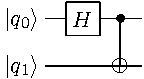
\includegraphics[width=0.28\textwidth]{figures/bell.pdf}
  \caption{Quantenschaltung zur Erzeugung von Bell-Zust\"anden}
  \label{fig:bell-circuit}
\end{figure}
Diese Schaltung kann genutzt werden um einen maximal verschr\"ankten Zustand zu erzeugen. Diese Zust\"ande werden Bell-Zust\"ande \textit{(Bell-State)} genannt \ref{eqn:bell-states}. Diese spielen eine zentralle Rolle in der Quanteninformation und sind unter anderem Grundbestandteil der Quantenteleportation und Quantenkryptographie.\\
Ein Zustand wird als verschr\"ankt bezeichnet, wenn er nicht in ein Produkt von Zust\"anden der einzelnen Bits zerlegt werden kann \cite{Homeister-2022}. Als maximal verschr\"ankt bezeichnet man den Zustand dann, wenn deren Bits maximal stark gekoppelt sind. D.h. jedes an diesem Zustand beteiligte Qubit, wird stets das selbe Ergebnis liefern. Ebenso muss der Einfluss der Messung dieser einzelnen Qubits auf das endg\"ultig gemessene Ergebnis gleich sein.
\begin{equation}
  \begin{aligned} \label{eqn:bell-states}
    |\beta_{00}\rangle = \frac{|00\rangle + |11\rangle}{\sqrt{2}}\\
    |\beta_{01}\rangle = \frac{|01\rangle + |10\rangle}{\sqrt{2}}\\
    |\beta_{10}\rangle = \frac{|00\rangle - |11\rangle}{\sqrt{2}}\\
    |\beta_{11}\rangle = \frac{|01\rangle - |10\rangle}{\sqrt{2}} 
  \end{aligned}
\end{equation}
Die Schaltung \ref{fig:bell-circuit} ist von links nach rechts zu lesen und enth\"alt bisher nur zwei Qubits, ein Hadamard-Gatter und ein $CX$-Gatter. Die geraden Linien sollen den Zeitablauf der Qubits darstellen. Um nun das Ergebnis dieser einzelnen Qubits zu erhalten m\"ussen diese gemessen und das Ergebnis auf klassische Bits \"ubertragen werden. Dazu muss die Schaltung folgenderma\ss en erweitert werden \ref{fig:bell-measured}.
\begin{figure}[h]
  \centering
  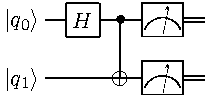
\includegraphics[width=0.38\textwidth]{figures/bell-measured.pdf}
  \caption{Messen von Qubits in der Schaltung zur Ereugung von Bell-Zust\"anden}
  \label{fig:bell-measured}
\end{figure}
Das neu hinzugekommene Symbol steht nun f\"ur eine Messung. Das Ergebnis dieser Messung wird in einem klassischen Bit gespeichert, doppelte Linien stehen in Quantenschaltungen also f\"ur klassische Bits.\\\\
Es gibt eine Menge an Schaltungen die interessante Probleme l\"osen oder Algorithmen implementieren, z.B. die Implementierung des Bernstein-Vazirani Problems \cite{Du_2001}. Oder die Implementierung des bekannten Quantensuchalgorithmus von Grover \cite{Figgatt_2017}. All diese Schaltungen sind unterschiedlich aufgebaut haben aber einige Gemeinsamkeiten, sie sind azyklisch und erlauben somit keine R\"uckf\"uhrung. F\"ur die Schaltungen gilt auch, dass das Zusammenf\"uhren der Qubits ohne Gatter oder das Kopieren der Qubits nicht erlaubt ist \cite{nielsen_chuang_2010}.
